% !TEX TS-program = pdflatex
% !TEX encoding = UTF-8 Unicode

% This is a simple template for a LaTeX document using the "article" class.
% See "book", "report", "letter" for other types of document.

\documentclass[11pt]{article} % use larger type; default would be 10pt

\usepackage[utf8]{inputenc} % set input encoding (not needed with XeLaTeX)

%%% Examples of Article customizations
% These packages are optional, depending whether you want the features they provide.
% See the LaTeX Companion or other references for full information.
\usepackage{float}

%%% PAGE DIMENSIONS

\usepackage{geometry} % to change the page dimensions
\geometry{margin=2cm,margin=2cm}
%\geometry{a4paper} % or letterpaper (US) or a5paper or....
% \geometry{margin=2in} % for example, change the margins to 2 inches all round
% \geometry{landscape} % set up the page for landscape
%   read geometry.pdf for detailed page layout information

\usepackage{graphicx} % support the \includegraphics command and options

% \usepackage[parfill]{parskip} % Activate to begin paragraphs with an empty line rather than an indent

%%% PACKAGES
\usepackage{booktabs} % for much better looking tables
\usepackage{array} % for better arrays (eg matrices) in maths
\usepackage{paralist} % very flexible & customisable lists (eg. enumerate/itemize, etc.)
\usepackage{verbatim} % adds environment for commenting out blocks of text & for better verbatim
\usepackage{subfig} % make it possible to include more than one captioned figure/table in a single float
% These packages are all incorporated in the memoir class to one degree or another...

%%% HEADERS & FOOTERS
\usepackage{fancyhdr} % This should be set AFTER setting up the page geometry
\pagestyle{fancy} % options: empty , plain , fancy
\renewcommand{\headrulewidth}{0pt} % customise the layout...
%\lhead{}\chead{}\rhead{}
%\lfoot{}\cfoot{\thepage}\rfoot{}

\fancyhead[LE,RO]{\textit{M1if - UCBL 2019-2020}}% efface le contenu de l'en-tete
%\fancyfoot{}% efface le contenu du pied de page
\fancyfoot[R,RO]{\textit{Rapport de POM de Pierre-Henri Chupin et Solomon Maria}}%Rapport deTER de


\fancyhf{} % Start with clearing everything in the header and footer
% Set the right side of the footer to be the page number
\fancyfoot[R]{\thepage}

% Redefine plain style, which is used for titlepage and chapter beginnings
% From https://tex.stackexchange.com/a/30230/828
\fancypagestyle{plain}{%
    \renewcommand{\headrulewidth}{0pt}%
    \fancyhf{}%
    \fancyfoot[L]{\thepage}%
}




%%% SECTION TITLE APPEARANCE
\usepackage{sectsty}
\allsectionsfont{\sffamily\mdseries\upshape} % (See the fntguide.pdf for font help)
% (This matches ConTeXt defaults)


%%% ToC (table of contents) APPEARANCE
\usepackage[nottoc,notlof,notlot]{tocbibind} % Put the bibliography in the ToC
\usepackage[titles,subfigure]{tocloft} % Alter the style of the Table of Contents
\renewcommand{\cftsecfont}{\rmfamily\mdseries\upshape}
\renewcommand{\cftsecpagefont}{\rmfamily\mdseries\upshape} % No bold!

%%% END Article customizations

%%% The "real" document content comes below...

\title{Modélisation distribuée d’un jeu stratégique : 
 \\ Cas d'une variante du jeu de dames}
\author{CHUPIN Pierre-Henri \\ SOLOMON Maria}
\date{} % Activate to display a given date or no date (if empty),
         % otherwise the current date is printed 

\begin{document}
\maketitle

\begin{abstract}
Abstract
Ce document décrit notre projet ayant pour  but  de  créer  une modélisation distribuée et de l'appliquer à un cas concret qui sera une variante du jeu de dames. Cela permettra de créer des stratégies pour des jeux et de comprendre mieux comment fonctionne la modélisation distribuée. Une démarche détaillée sur nos réalisations ainsi que les limitations de notre travail y seront présentées.  \\
Mots-clés: Intelligence artificielle distribuée, intelligence artificielle centralisée, stratégie, recherche de risque
\end{abstract}



\section{Introduction}
Le sujet de notre Projet d’Orientation en Master(POM) est Modélisation distribuée d’un jeu stratégique: Cas d'une variante du jeu de dames. Il s'inscrit dans le cadre du second semestre de Master 1 informatique de Lyon 1 et dans l'optique de poursuivre en Master IA. Pour ce projet nous avons pu compter sur notre encadrant Aknine Samir appartenant à l'équipe Systèmes Multi-Agents de LIRIS dont les axes de recherches s’inscrivent dans le domaine de l'intelligence artificielle. 
L’Intelligence artificielle Distribuée (IAD) vise à combler les lacunes de l’approche classique de l’IA en proposant la distribution de l’expertise sur un groupe d’agents.
Elle se définit comme la branche de l’IA qui s’intéresse à la modélisation de comportement intelligent d’un ensemble d’agents opérant collectivement et de façon décentralisée pour parvenir à un objectif global.
La création d’un jeu de dames géré par une intelligence artificielle distribuée ainsi que l'implémentation d’un ensemble de stratégies collectives restent une problématique assez actuelle et s’ouvre à plusieurs types de solutions comme l’algorithme MinMax. 

\section{Etat de l'art}
L’Intelligence artificielle distribuée(IAD)
L’IAD s’intéresse à des comportements intelligents qui sont le produit de l’activité coopérative de plusieurs agents. Elle représente une branche de l'intelligence artificielle dont le but est de créer des systèmes décentralisés, généralement multi-agents, capables de coopérer et de se coordonner. L'intelligence artificielle distribuée étudie les techniques permettant à des agents autonomes d'interagir, et les moyens de répartir un problème entre ces agents. Ces techniques sont inspirées des structures complexes de certaines sociétés d'insectes comme les fourmis. Un des domaines d'application de l'IAD est la coordination d'agents autonomes mobiles (comme les avions ou les voitures) - qui doivent apprendre à s'éviter tout en ayant des contraintes de trajet et de temps. 
Dans un système multi-agents géré par ce type d’IA on va trouver une communauté d’agents autonomes qui évoluent dans un environnement commun, selon des modes parfois complexes de coopération, de concurrence voire de conflit, pour aboutir à un objectif global. Un agent est un logiciel ou un matériel capable de capter de l’information, d’agir " rationnellement " en fonction des données récupérées et de déclencher une action pour optimiser ses chances de succès.
Un agent peut réagir en temps réel et en fonction de l’environnement. Lorsque cela s’avère nécessaire par la complexité de l’objectif à atteindre, les agents intelligents sont intégrés dans des systèmes multi-agents constitués d’une somme d’agents autonomes, mais reliés et collaborant entre eux. 
Ces agents constituent un système complexe qui comprend une intelligence que l’on pourrait qualifier de collective.

\subsection{L’Intelligence artificielle centralisée}

L’approche classique de l’Intelligence Artificielle(IA) suppose une fondation sur une centralisation de l’expertise au sein d’un seul et unique système expert. De plus, tous les entités qui font partie de ce système central en sont dépendantes, tous les décisions et les stratégies sont pris par le système.

\subsection{L’algorithme MinMax}

Minimax est un algorithme décisionnel , généralement utilisé dans un jeu au tour par tour, à deux joueurs . Son but est de trouver le prochain coup optimal.
L'objectif est de trouver le meilleur coup pour le joueur. Pour ce faire, nous pouvons simplement choisir le nœud avec le meilleur score d’évaluation. Pour rendre le processus plus intelligent, nous pouvons également regarder de l’avant et évaluer les mouvements de nos adversaires potentiels.
Pour chaque mouvement, nous pouvons prévoir autant de mouvements que notre puissance de calcul le permet. L’algorithme suppose que l’adversaire joue de manière optimale.
Techniquement, nous commençons par le nœud racine et choisissons le meilleur nœud possible. Nous évaluons les nœuds en fonction de leurs scores d’évaluation. Dans notre cas, la fonction d’évaluation peut attribuer des scores aux seuls nœuds de résultats (feuilles).
Par conséquent, nous atteignons récursivement les feuilles avec des scores et propageons les scores en arrière.


\section{Implementation}
Dans cette étape nous allons présenter l’interface graphique des dames, les règles qu’on a choisi, décrire en détails la mise en place de l’algorithme MinMax, le calcul du meilleur coup  d’une pièce et mesurer le risque de son coup. On va également aller plus loins sur les potentielles améliorations ainsi que les limitations de nos réalisations.



\subsection{Le règles du jeu}

Notre modélisation se base sur le jeux de dames classique avec quelques changements qui permettent d'avoir des comportements différents et plus intéressants. 
Voici l’ensemble des règles qu’on a implémenté: 
\begin{itemize}
\item Un plateau carré de 10 cases sur 10
\item 20 pions blancs et 20 pions noir
\item Un pion se déplace d’une case à la fois
\item 2 IAs qui joueront à tour de rôle de 1 à 3 pièces (nombre maximal qui peut être changé avant de lancer une partie)
\item Un pion devient une dame quand il va atteindre le bout du territoir de l’ennemi
\item Une dame se déplace de 1 jusqu’à 3 cases maximum 
\item La prise d’une pièce est obligatoire, que ça soit en arrière ou en avant 
 \item La prise multiple est possible et reste également obligatoire
\item une partie est gagnée quand:
\begin{itemize}
\item si toutes les pièces adverses sont prises
\item si l'adversaire a toutes ses pièces bloquées
\end{itemize}
\item une partie est nul quand:
\begin{itemize}
\item s'il y a 30 coups sans prise
\end{itemize}
\end{itemize}

\section{Modélisation du jeu de dame}

Nous avons opté pour une conceptualisation distribuée et décentralisée où 2 IAs principales vont coordonner le tour de rôle de chaque équipe ainsi que le nombre maximum de pions qui vont se déplacer. Le choix de l’action reste aux pions. Chaque pion sera déplacé en fonction du coup le moins risqué qu’il a à sa disposition, ce qui est assuré par l’algorithme MinMax. 

\subsection{Calcul du meilleur coup pour une pièce}

Chaque pion a la possibilité de choisir une action à faire qu’il va prendre en fonction de son propre environnement. De plus, il va mesurer tous ses possibilités et va exécuter le coup le plus avantageux pour lui. 

Dans la Figure 1, le pion a devant lui 2 cases libres. Dans ce cas on fait un tirage aléatoire pour choisir une case. 
Dans la Figure 2, l’un des pions marrons a toujours le choix entre les 2 cases libres sauf que cette fois on va mettre en priorité de ne pas rester coincé. Donc ce pion va abandonner la stratégie initiale aléatoire et ne vas pas risquer de se faire bloqué en choisissant l’autre case libre sans ce risque.

Dans la Figure 3 le pion a un choix égale de prise. On va opter dans ce cas pour une prise dans la direction du territoir de l’ennemi.

La Figure 4 représente le cas où le pion peut prendre 1 ou 2 ennemis. Il va choisir le coup le plus avantageux sans tenir compte de la direction d'avancement comme dans la Figure 3. 
 
\begin{figure}[!htb]
\minipage{0.22\textwidth}
	\caption{  }
	\label{fig_sim}
	{
	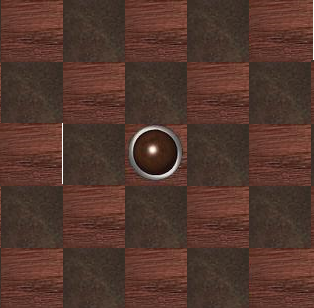
\includegraphics[width=\linewidth]{1Q}
	\label{paysage}
	}
\endminipage\hfill
\minipage{0.22\textwidth}
	%\caption{ l’un des pions marrons a toujours le choix entre les 2 cases libres sauf que cette fois on va mettre en priorité de ne pas rester coincé.}
	\caption{  }
	\label{fig_sim}
	%\centering
	%\subfloat[Donc ce pion va abandonner la stratégie initiale aléatoire et ne vas pas risquer de se faire bloqué en choisissant l’autre case libre sans ce risque.]
	{
	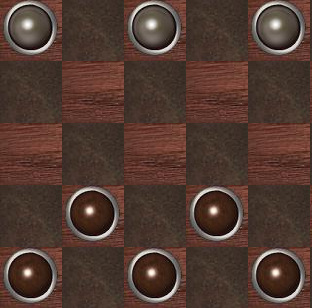
\includegraphics[width=\linewidth]{2}
	\label{paysage}
	}
\endminipage\hfill
\minipage{0.22\textwidth}
	%\caption{le pion à un choix égale de prise.}
	\caption{  }
	\label{fig_sim}
	%\centering
	%\subfloat[ On va opter dans ce cas pour une prise dans la direction du territoir de l’ennemi.]
	{
	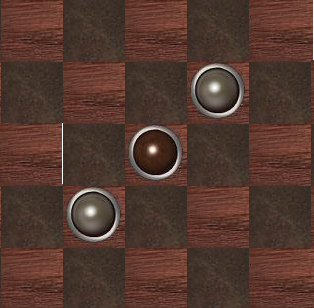
\includegraphics[width=\linewidth]{3}
	\label{paysage}
	}
\endminipage\hfill
\minipage{0.22\textwidth}
	\caption{  }
	\label{fig_sim}
	%\centering
	%\subfloat[ Il va choisir le coup le plus avantageux sans tenir compte de la direction d'avancement comme dans la Figure 3.]
	{
	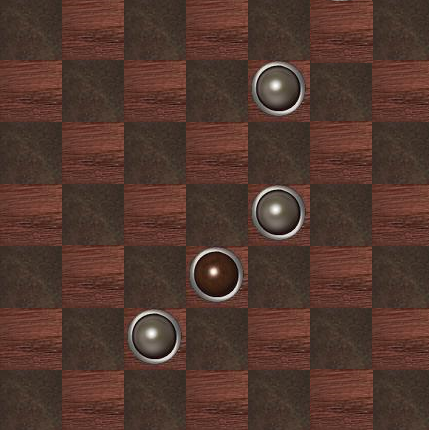
\includegraphics[width=\linewidth]{4}
	\label{paysage}
	}
\endminipage
\end{figure}

\subsection{Calcul du coup risqué pour une pièce}

En s’inspirant de l’algorithme MinMax nous avons décidé de calculer pour chaque pièce le coup le moins risqué qu’elle peut effectuer. Avec l’algorithme qu’on a mis en place, il est possible de prévoir un coup en tenir compte de 2 prochains coups en avance. 
Il y a plusieurs approches pour apprécier le score d’un coup
\begin{itemize}
\item si une pièce a le choix de se déplacer, on va tenir compte si au tour suivant elle ne se fait pas prendre
\begin{itemize}
\item si elle sera prise, elle choisira l’autre option moins risqué s’il existe
\item sinon elle avance
\end{itemize}
\item si une pièce peut prendre un ou plusieurs ennemis mais qu’elle se fait mangée au tour suivant, on va considérer ce coup risqué si le nombre de pions mangés est plus grande ou égal au nombre de pions que l’ennemi va prendre à son tour
\item si aucune possibilité de déplacement non risqué est possible, alors il se déplace vers une position risquée
\end{itemize}

Un compteur a été ajouté pour éviter les situations bloquantes où une pièce se trouve déjà sur une position risquée. Son but est de compter le nombre de risque avant de tester des déplacements et de la comparer avec le nombre de risque retrouvé après un déplacement. 

\subsection{Strategies collectives}

Une remarque intéressante à faire serait que le déplacement sans risque d’une pièce peut créer des risques sur une autre pièce ailleurs sur le plateau. Par conséquent, toutes les pièces d'une même équipe vont coopérer entre elles afin de tester si un coup en particulier rendrait une pièce vulnérable à la prise adversaire. Cela est possible en testant toutes les pièces pour chaque tentative de déplacement et à chaque fois aller plus loin qu'un seul coup.  
La complexité va augmenter vite à chaque fois qu’on va calculer un coup de plus en avance, étant donnée qu’on va aller plus en profondeur de l’arbre MinMax de possibilités.
Le problème étant que l'arbre devient extrêmement grand très rapidement.


\subsection{Implémentation de l’algorithme}

A chaque fois qu'on prévoit de déplacer une pièce, nous fabriquons un arbre avec toutes les possibilitées de mouvement et on descend le plus possible en profondeur à l’aide d’une fonction récursive. Le but est de tester si ce mouvement sera risqué ou non. 
Comme la simulation de l’arbre entier est très coûteux en mémoire, nous limitons notre parcours en profondeur et la façon dont nous cherchons dans l'arbre afin d’optimiser. Au lieu de créer tout l'arbre puis de chercher dedans, on va petit à petit le créer et on va s’arrêter dès qu'un mouvement satisfaisant est trouvé. 
La démarche à suivre sera de prendre les pièces qui ont un choix de déplacement et tester si après avoir réalisé ce déplacement elles risquent de se faire prendre par l'adversaire.
Si c'est le cas alors les pièces ne bougent pas. Au contraire, si elles peuvent se déplacer sans risque alors elles avancent et nous arrêtons l’avancement de l’arbre. 
Cela implique des limites car il y a certains cas où un coup sans risque par rapport à un autre est plus efficace.

\subsection{Interface graphique}

Nous avons donné un aspect graphique au jeu afin de mieux voir ce qui se passe pendant le déroulement du programme. Dans l’annexe 1 à gauche il y a le plateau de dames accompagné d’une échelle horizontale avec des lettres et une échelle verticale avec de chiffres pour identifier mieux les cases. 
A droite nous disposons d’un panneau de debug qui permet de voir à chaque tour qui quelles pièces se sont déplacées. Dans la Figure 5 on peut voir un extrait du panneau. La police gris représente les pions blancs et la police rouge les autres pions adverses. “Ph x” signifie le ième tour sachant que pendant un tour les 2 équipes vont faire leurs mouvements. “4E” et “6C” sont les anciennes positions de ces 2 pions et  “5F”, “7B” sont leurs nouvelles positions. “(D)” ou “(P)” signifie le type de mouvement, D pour le déplacement et P pour la prise.

\begin{figure}[!ht]
\caption{exemple.}
\label{fig_sim}
\centering
{
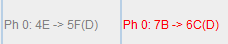
\includegraphics[width=2in]{6}
\label{paysage}
}
\end{figure}

\subsection{Améliorations possibles et limitations}
Une amélioration est possible dans la recherche de risque. Nous aurions pu aussi prendre en compte le nombre de pièces perdues après un mouvement risqué pour faire un meilleur choix de déplacement.
De plus, nous aurions pu essayer d'aller plus en profondeur et voir plus loin dans le risque, mais cela aurait ajouté beaucoup de complexité et aurait ralenti notre algorithme mais l'aurait rendu bien plus solide et moins risqué. Le problème étant que l'arbre devient extrêmement grand très rapidement.



\section{Conclusion}

Nous avons bien créé une conceptualisation distribuée et adaptée à un jeu de dame personnalisé. Les stratégies implémentées sont performantes étant donnée qu’elles tiennent compte du meilleur coup de la pièce et estiment en même temps le risque d’un tel mouvement. De plus, les pièces peuvent facilement coopérer entre elles et minimiser le risque de toute l’équipe, ce qui les a rendu plus indépendantes.
Le choix d’un algorithme inspiré par le MinMax, nous a limité le nombre de coups possibles à prévoir en avance. Par conséquent, plus on améliore le calcul du coup optimal, plus on augmente dans la complexité.
Ce projet à permis de mieux voir la puissance et l'importance des modélisations distribuées dans le cas où il faut simuler plusieurs agents qui doivent communiquer entre eux pour avancer dans un environnement aux règles stricts et atteindre un objectif commun.

\section{Annexes}
\begin{figure}[!ht]
\caption{exemple de l'interface complet}
\label{fig_sim}
\centering
{
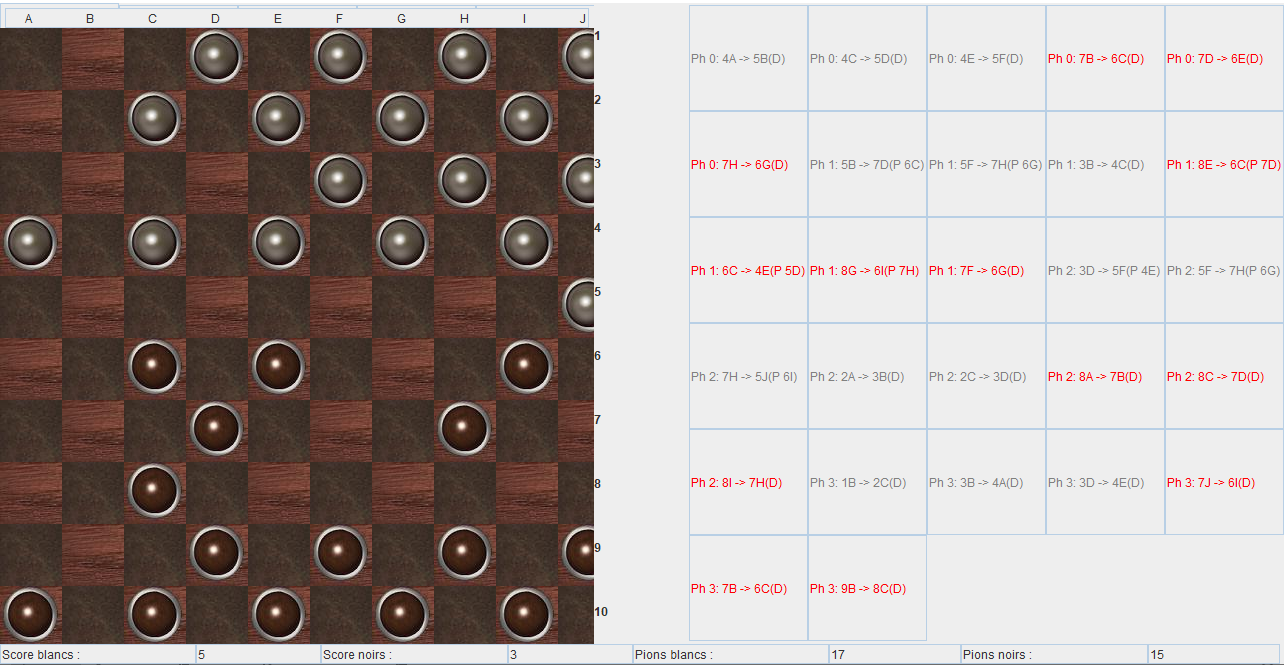
\includegraphics[width=6in]{5}
\label{paysage}
}
\end{figure}

\end{document}
